\documentclass[11pt, oneside]{article} 
\usepackage{geometry}
\geometry{letterpaper} 
\usepackage{graphicx}
	
\usepackage{amssymb}
\usepackage{amsmath}
\usepackage{parskip}
\usepackage{color}
\usepackage{hyperref}

\graphicspath{{figures/}{/Users/telliott/Github-Math/figures/}}
% \begin{center} \includegraphics [scale=0.4] {gauss3.png} \end{center}

\title{Archimedes' Quadrature (Lemma)}
\date{}

\begin{document}
\maketitle
\Large

%[my-super-duper-separator]

Let the parabola be $y=x^2$ with points $P=(v,v^2)$ and $Q=(u,u^2)$.  The secant $PQ$ has equation $y = (u+v)x - uv$ (check both points).  The tangent $QM$ has equation $y = 2ux - u^2$ (ditto).
\begin{center} 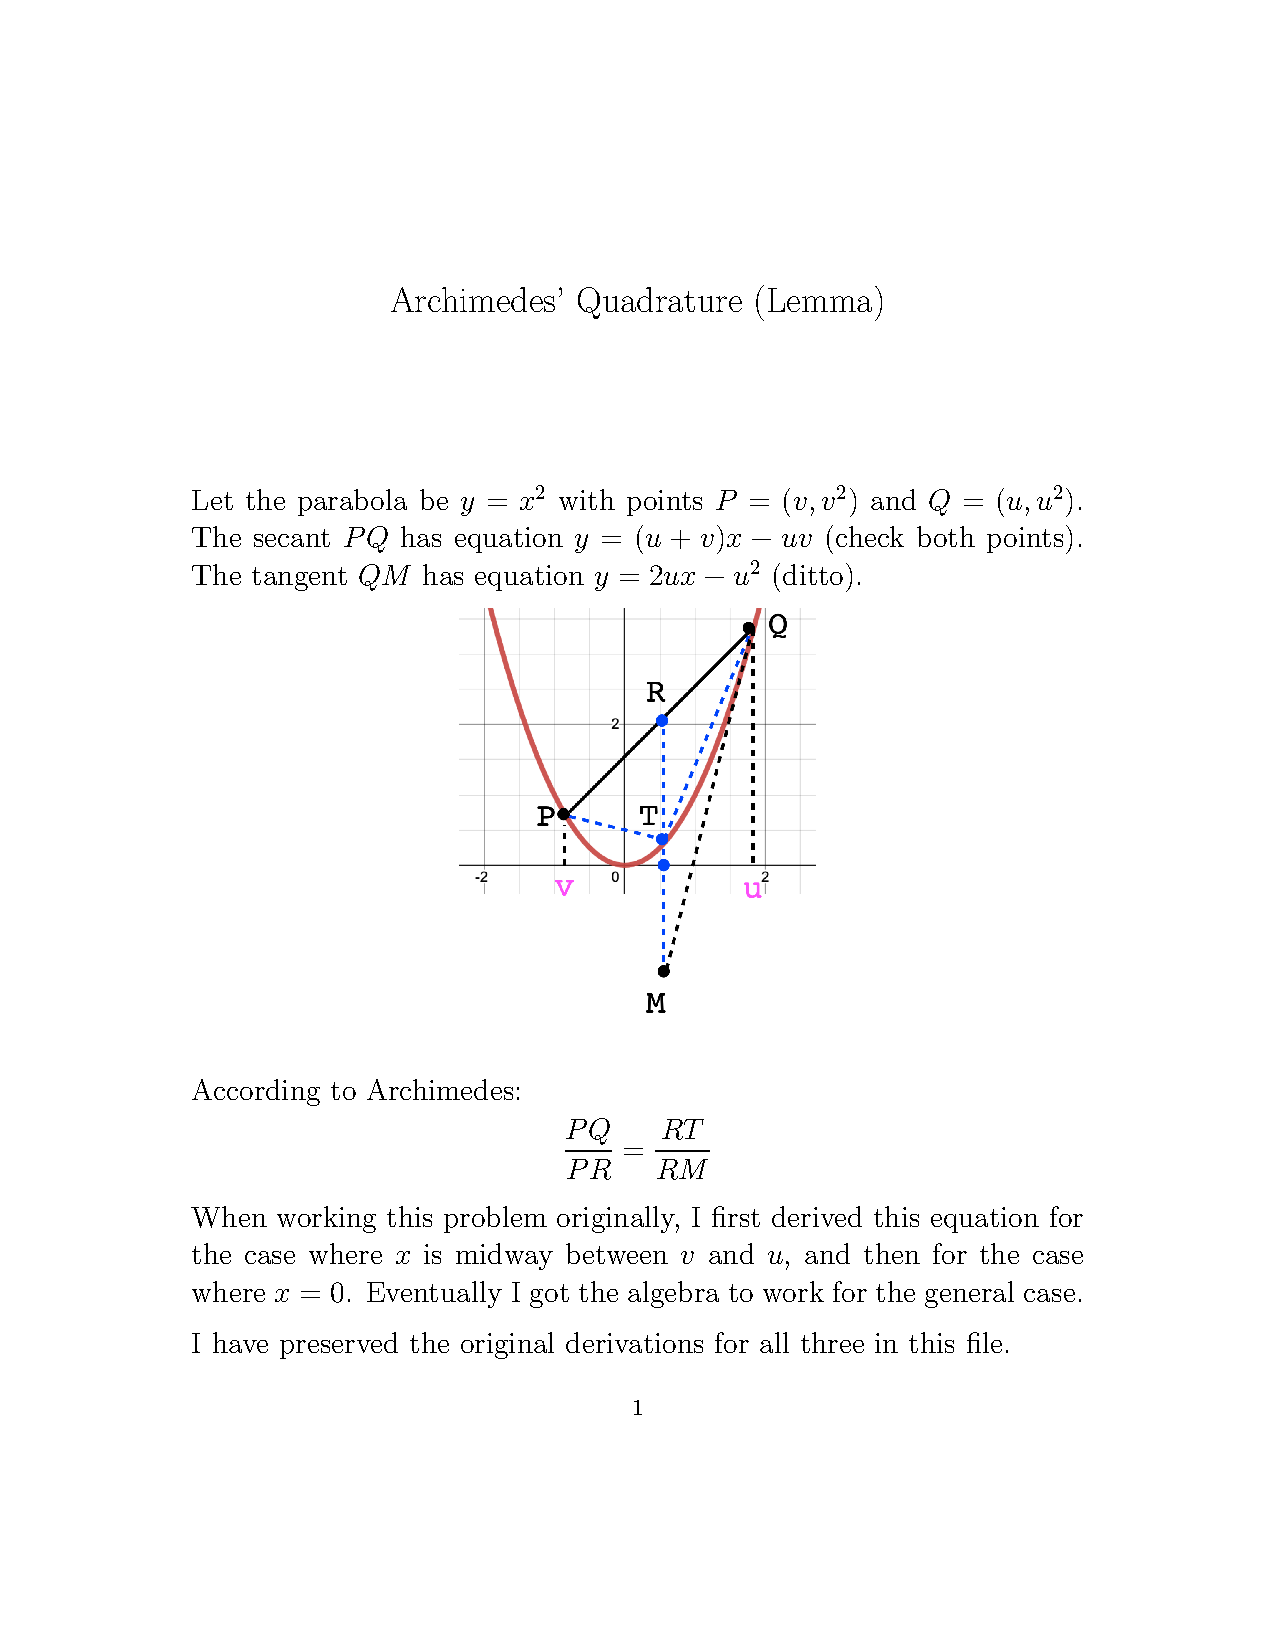
\includegraphics [scale=0.4] {qq3.png} \end{center}

According to Archimedes:
\[ \frac{PQ}{PR} = \frac{RT}{RM} \]

When working this problem originally, I first derived this equation for the case where $x$ is midway between $v$ and $u$, and then for the case where $x=0$.  Eventually I got the algebra to work for the general case.

I have preserved the original derivations for all three in this file.

\subsection*{meeting tangents}
The tangent through $Q$ has slope $2u$ and has the equation
\[ y = 2ux + y_0 \]
\[ u^2 = 2u^2 + y_0 \]
\[ y_0 = -u^2 \]
so
\[ y = 2ux - u^2 \]
similarly, the tangent through $P$ is
\[ y = 2vx - v^2 \]

Let us consider the point $M$ where the two tangents meet.  
\[ 2ux - u^2 = 2vx - v^2 \]
\[ x = \frac{u^2 - v^2}{2(u - v)} = \frac{u+v}{2} \]
This is the $x$-value halfway between $P$ and $Q$.  The $y$-value is
\[ M_y = 2u \cdot (u+v)/2 - u^2 \]
\[ = uv \]
And in this example, $v < 0$ so $M_y < 0$ as well.

The point $T$ is on the curve $y=x^2$:
\[ T_y = (\frac{u+v}{2})^2 = \frac{(u+v)^2}{4} \]

The point $R$ is halfway along the secant  so as we said before:
\[ R_y = \frac{u^2 + v^2}{2} \]

Alternatively, the secant $PQ$ has slope $u+v$ (see above)
\[ y = (u+v)x + y_0 \]
and it goes through $Q$ so
\[ u^2 = (u+v)u + y_0 \]
\[ y_0 = - uv \]
The equation of the secant is
\[ y = (u+v)x - uv \]
(Since $v < 0$, the intercept $y_0 > 0$).

So the value of $y$ at $x = (u+v)/2$ is
\[ R_y = \frac{(u+v)^2}{2} - uv = \frac{u^2 + v^2}{2} \ \ \ \ \ \checkmark \]

\begin{center} 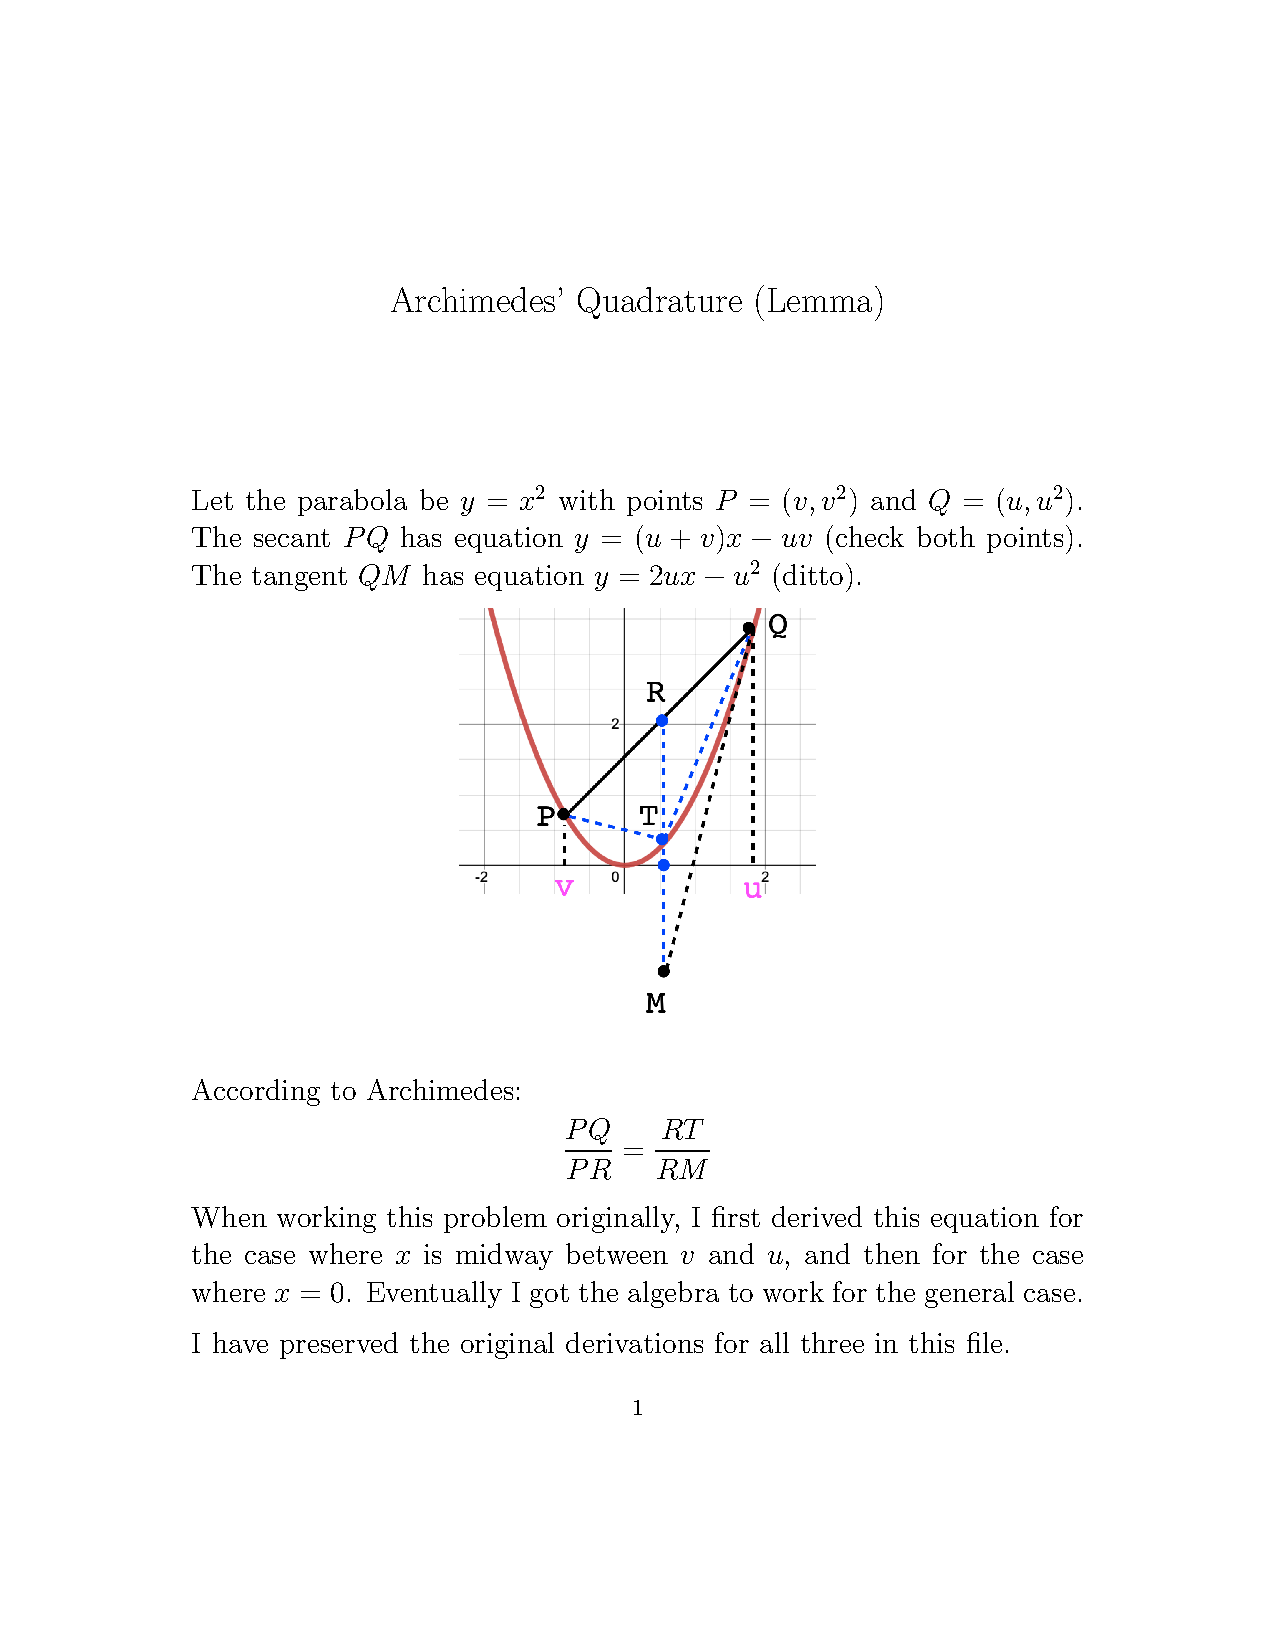
\includegraphics [scale=0.4] {qq3.png} \end{center}
The extensions give three points with the same $x$ and corresponding $y$-values:
\[ M_y = uv, \ \ \ \ \ R_y =\frac{u^2 + v^2}{2},  \ \ \ \ \  T_y = \frac{(u+v)^2}{4} \]
\[ R_y - T_y = \frac{u^2 + v^2}{2} - \frac{(u+v)^2}{4} \]
\[ = \frac{u^2}{4} - \frac{uv}{2} + \frac{v^2}{4} = \frac{(u-v)^2}{4}  \]

Similarly
\[ T_y - M_y =  \frac{(u+v)^2}{4} - uv \]
\[ = \frac{(u+v)^2 - 4uv}{4} = \frac{(u-v)^2}{4}  \] 

We have shown that
\[ R_y - T_y = T_y - M_y \]
\[ 2T_y = R_y + M_y \]
\[ T_y = \frac{R_y + M_y}{2} \]

\subsection*{other verticals}
Anticipating what we will need for Archimedes second proof, we think about what happens if we slide the vertical line $RTM$ over horizontally.  The claim is that the ratios go like
\[ \frac{RT}{RM} = \frac{PR}{PQ} \]
and we do have that for the midway point.

Probably the easiest second case is if $RTM$ becomes the $y$-axis, $x = 0$.

The equation of the secant $PQ$ is
\[ y = (u+v)x - uv \]
The equation of the tangent through $Q$ is
\[ y = 2ux - u^2 \]

The $y$-intercepts are $R_y' = -uv$ and $M_y' = -u^2$.  $T_y'$ is just zero.

The one length that will not change is $PQ$.  The square is:
\[ PQ^2 = (u^2 - v^2)^2 - (u - v)^2 \]
We can actually do something with that because the first term is
\[ (u+v)(u-v)(u+v)(u-v) \]
so
\[ PQ^2 = (u+v)^2 \cdot (u-v)^2 - (u - v)^2 \]
\[ = (u-v)^2 \cdot \ [ 1 + (u+v)^2 \ ] \]

The easy lengths are:
\[ RT = -uv \]
\[ RM = -uv - (-u^2) \]
\[ = u(u - v) \]
and the ratio is $RT/RM$
\[ \frac{-v}{u - v} \]
which is positive, as all lengths should be.

The last one is the hardest:
\[ PR^2 = (-uv - v^2)^2 + (0-v)^2 \]
We factor $(-1)^2$ from the first term
\[ = (uv + v^2)^2 + v^2 \]
and then out comes $v^2$:
\[ = \ [ \ v^2 \ [ \ 1 + (u + v)^2 \ ] \]
and now we see it!
The ratio is $PR/PQ$ except we have the square
\[ \frac{ \ v^2 \ [ \ 1 + (u + v)^2 \ ]}{(u-v)^2 \cdot \ [ 1 + (u+v)^2} \]
After cancelation and the square root we have that the ratio is
\[ PR/PQ = \pm \frac{v}{u - v} \]

As we said, lengths are positive.  $v < 0$ and the denominator is positive so we take the negative root:
\[ = -\frac{v}{u - v} \]
which is a match.

Since the ratios are also equal for this second vertical it is an encouragement to see if we can make them work for all of them, as Archimedes will claim.  Can we re-work this proof for arbitrary $x$?

Suppose that $x = k(u+v) = w$.  We have that 
\[ R_y = (u+v)w - uv \]
\[ = uw + vw - uv \]
\[ T_y = w^2 \]
\[ M_y = 2uw - u^2 \]

\[ RT = uw + vw - uv  - w^2 \]
\[ = (w - v)(u - w) \]
and
\[ RM =  uw + vw - uv - 2uw + u^2 \]
\[ = vw - uv - uw + u^2 \]
looking for $(u - w)$:
\[ = (u - w) (u - v) \]

The ratio $RT/RM$ is
\[ \frac{w - v}{u - v} \]

$PQ^2$ stays the same.
\[ PQ^2 = (u-v)^2 \cdot \ [ 1 + (u+v)^2 \ ] \]

And the last one is
\[ PR^2 = \ [ \ (u+v)w - uv - v^2 \  ]^2 + (w-v)^2 \]
\[ = \ [ \ (w - v)(u+v) \ ]^2 + (w-v)^2 \]
\[ = (w-v)^2 \ [ \ 1 + (u+v)^2 \ ] \]
So $PR/PQ$ does simplify.  The ratio is just ($\pm$):
\[ = \frac{w-v}{u-v} \]
It was a great idea to write everything with $w$!

We confirm that this ratio is invariant:
\[ \frac{PR}{PQ} = \frac{RT}{RM} \]
\begin{center} 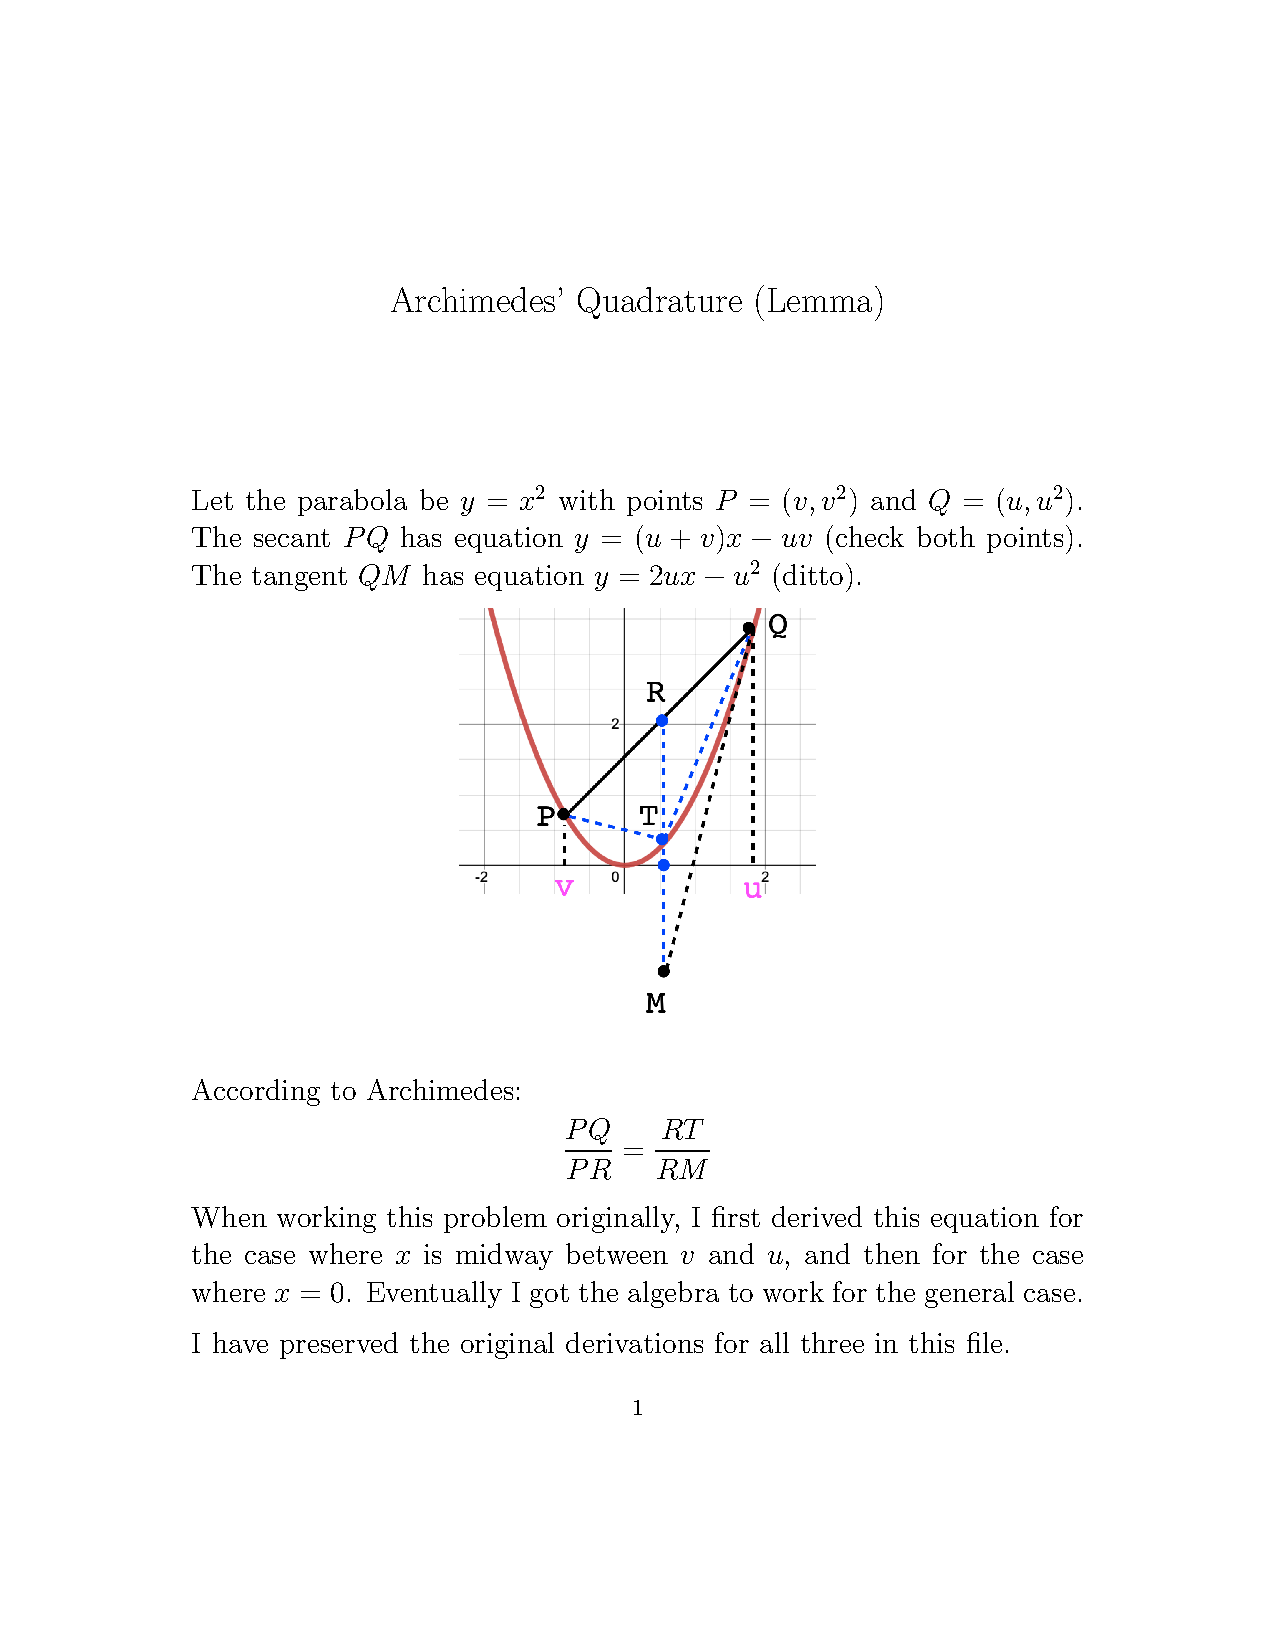
\includegraphics [scale=0.4] {qq3.png} \end{center}

After six pages of algebra, it finally occurs to me that \emph{of course} this works, at least for $PR/PQ$.  The fraction of the length of $PQ$ taken up by $PR$ is exactly the same as the fraction of $u-v$ taken up by $u-w$ since $PQ$ is a straight line.

The wonderful part is that it works for $RT/RM$ as well.


So then let $w$ lie somewhere between $v$ and $u$, and then $T_y = w^2$.  We can get $R$ and $M$ from the equations above as $R_y = (u+v)w - uv$ and $M_y = 2uw - u^2$.

The first ratio is *
\[ \frac{PR}{PQ} = \frac{w-v}{u-v} \]
by similar triangles (bases and hypotenuses in same proportion).

Then the other ratio that we want to match it is $RT/RM$.
\[ |RT| = R_y - T_y = (u+v)w - uv - w^2 \]
\[ |RM| = R_y - M_y = (u+v)w - uv - 2uw + u^2 \]
\[ = vw - uv - uw + u^2 \]
We can be guided by the first ratio.  We want $(u-v)$ on the bottom.
\[ |RM| = u(u-v) + w(v - u) = (u-v)(u-w) \]
So then let's try to find $(u-w)$ on top
\[ |RT| =  (u+v)w - uv - w^2 \]
\[ = uw - uv + wv - w^2 \]
\[ = u(w - v) + w(v-w) = (u-w)(w-v) \]
Thus
\[ \frac{RT}{RM} = \frac{(u-w)(w-v)}{(u-v)(u-w)} = \frac{w-v}{u-v} = \frac{PR}{QR} \]
$\square$

* \emph{Proof} (additional).

The secant has equation $y = kx + y_0$ where $k = (u+v)$.  So $|RP|^2$
\[ = \Delta y^2 + \Delta x^2 = \ [ \ kw - y_0 - (k v - y_0) \ ]^2 + (w - v)^2 \]
\[ (k^2 + 1)(w - v)^2 \]
$|PQ|^2$ is exactly the same, with $u$ substituted for $w$.  So in the ratio of the square roots we have just $(w-v)/(u-v)$.

\end{document}